%%%%%%%%%%%%%%%%%%%%%%%%%%%%%%%%%%%%%%%%%
% Journal Article
% LaTeX Template
% Version 1.3 (9/9/13)
%
% This template has been downloaded from:
% http://www.LaTeXTemplates.com
%
% Original author:
% Frits Wenneker (http://www.howtotex.com)
%
% License:
% CC BY-NC-SA 3.0 (http://creativecommons.org/licenses/by-nc-sa/3.0/)
%
%%%%%%%%%%%%%%%%%%%%%%%%%%%%%%%%%%%%%%%%%

%----------------------------------------------------------------------------------------
%	PACKAGES AND OTHER DOCUMENT CONFIGURATIONS
%----------------------------------------------------------------------------------------

\documentclass[twoside]{article}

\usepackage{lipsum} % Package to generate dummy text throughout this template

\usepackage[sc]{mathpazo} % Use the Palatino font
\usepackage[T1]{fontenc} % Use 8-bit encoding that has 256 glyphs
\linespread{1.05} % Line spacing - Palatino needs more space between lines
\usepackage{microtype} % Slightly tweak font spacing for aesthetics

\usepackage[hmarginratio=1:1,top=32mm,columnsep=20pt]{geometry} % Document margins
\usepackage{multicol} % Used for the two-column layout of the document
\usepackage[hang, small,labelfont=bf,up,textfont=it,up]{caption} % Custom captions under/above floats in tables or figures
\usepackage{booktabs} % Horizontal rules in tables
\usepackage{float} % Required for tables and figures in the multi-column environment - they need to be placed in specific locations with the [H] (e.g. \begin{table}[H])
\usepackage{hyperref} % For hyperlinks in the PDF

\usepackage{lettrine} % The lettrine is the first enlarged letter at the beginning of the text
\usepackage{paralist} % Used for the compactitem environment which makes bullet points with less space between them

\usepackage{abstract} % Allows abstract customization
\renewcommand{\abstractnamefont}{\normalfont\bfseries} % Set the "Abstract" text to bold
\renewcommand{\abstracttextfont}{\normalfont\small\itshape} % Set the abstract itself to small italic text

\usepackage{titlesec} % Allows customization of titles
\renewcommand\thesection{\Roman{section}} % Roman numerals for the sections
\renewcommand\thesubsection{\Roman{subsection}} % Roman numerals for subsections
\titleformat{\section}[block]{\large\scshape\centering}{\thesection.}{1em}{} % Change the look of the section titles
\titleformat{\subsection}[block]{\large}{\thesubsection.}{1em}{} % Change the look of the section titles

\usepackage{fancyhdr} % Headers and footers
\pagestyle{fancy} % All pages have headers and footers
\fancyhead{} % Blank out the default header
\fancyfoot{} % Blank out the default footer
\fancyhead[C]{ESE650 Learning in Robotics $\bullet$ February 2014 $\bullet$ Project 2} % Custom header text
\fancyfoot[RO,LE]{\thepage} % Custom footer text

\usepackage[pdftex]{graphicx}
\usepackage{subfigure}
\usepackage{amsmath,amssymb,amsopn,amstext,amsfonts}
\usepackage{url}
\usepackage[usenames,dvipsnames]{color}
\usepackage{siunitx}
\graphicspath{{fig/}}
\newcommand{\red}[1]{\textcolor{red}{#1}}
\newcommand{\brown}[1]{\textcolor{brown}{#1}}
%----------------------------------------------------------------------------------------
%	TITLE SECTION
%----------------------------------------------------------------------------------------

\title{\vspace{-15mm}\fontsize{24pt}{10pt}\selectfont\textbf{Orientation Tracking}} % Article title

\author{
\large
\textsc{Chao Qu}\thanks{A thank you or further information}\\[2mm] % Your name
\normalsize University of Pennsylvania \\ % Your institution
\normalsize \href{mailto:quchao@seas.upenn.edu}{quchao@seas.upenn.edu} % Your email address
\vspace{-5mm}
}
\date{}

%----------------------------------------------------------------------------------------

\begin{document}


\maketitle % Insert title

\thispagestyle{fancy} % All pages have headers and footers

%----------------------------------------------------------------------------------------
%	ABSTRACT
%----------------------------------------------------------------------------------------

%\begin{abstract}
%
%\noindent Hey, I'm just an abstract. % Dummy abstract text
%
%\end{abstract}

%----------------------------------------------------------------------------------------
%	ARTICLE CONTENTS
%----------------------------------------------------------------------------------------

%----------------------------------------------------------------------------------------
%	INTRODUCTION
%----------------------------------------------------------------------------------------

\begin{multicols}{2} % Two-column layout throughout the main article text

\section{Introduction}
\lettrine[nindent=0em,lines=2]{O}rientation Tgracking

%----------------------------------------------------------------------------------------
%	PRE-PROCESSING
%----------------------------------------------------------------------------------------

\section{Pre-processing}
The raw IMU data we get is 10-bit ADC values, which technically ranges from 0 to 1023. Since it's difficult to use those values directly in our filter, we have to convert them so that they have real-world physical units and meanings. Our goal here is to convert the readings from the micro-controller to acceleration with a unit of \si{m/s^2} and angular velocity with a unit of \si{\radian/s}.
%\begin{figure}[H]
%  \centering
%  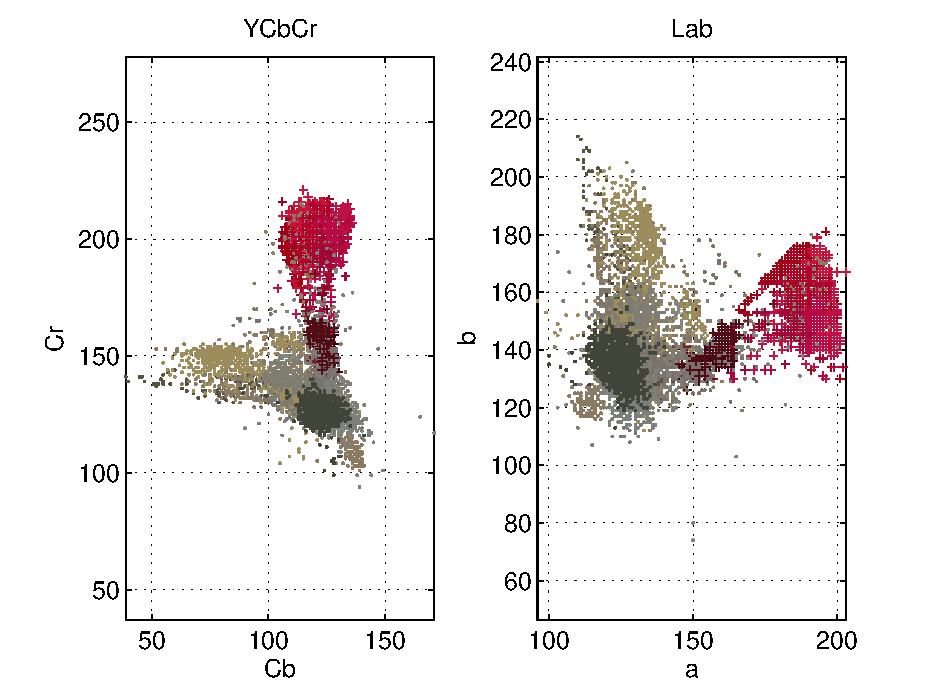
\includegraphics[width=\columnwidth]{cspace_2d.pdf}
%    \caption{2D scatter plot on the 2 color channels of L*a*b and YCbCr}
%    \label{fig:cspace_2d}
%\end{figure}

%\begin{figure}[H]
%  \centering
%  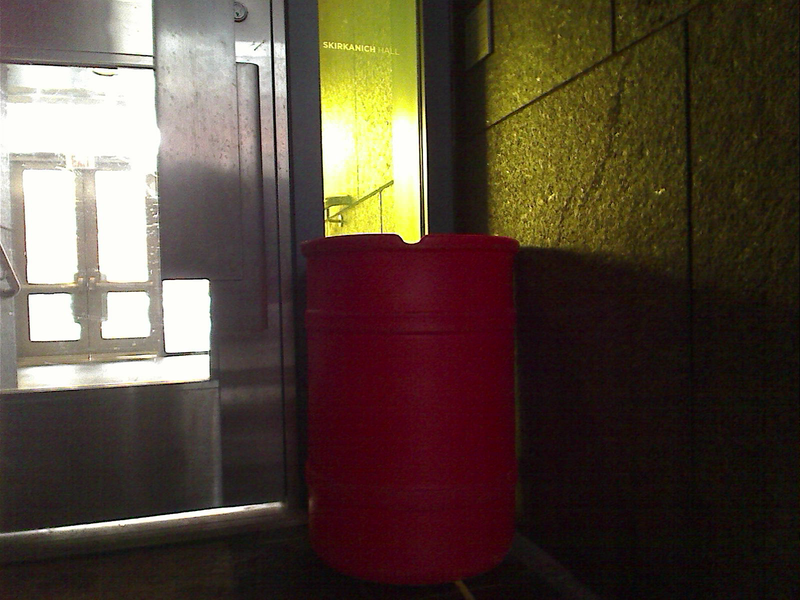
\includegraphics[width=0.4\columnwidth]{barrel_dark.png}
%  \;\;\;
%  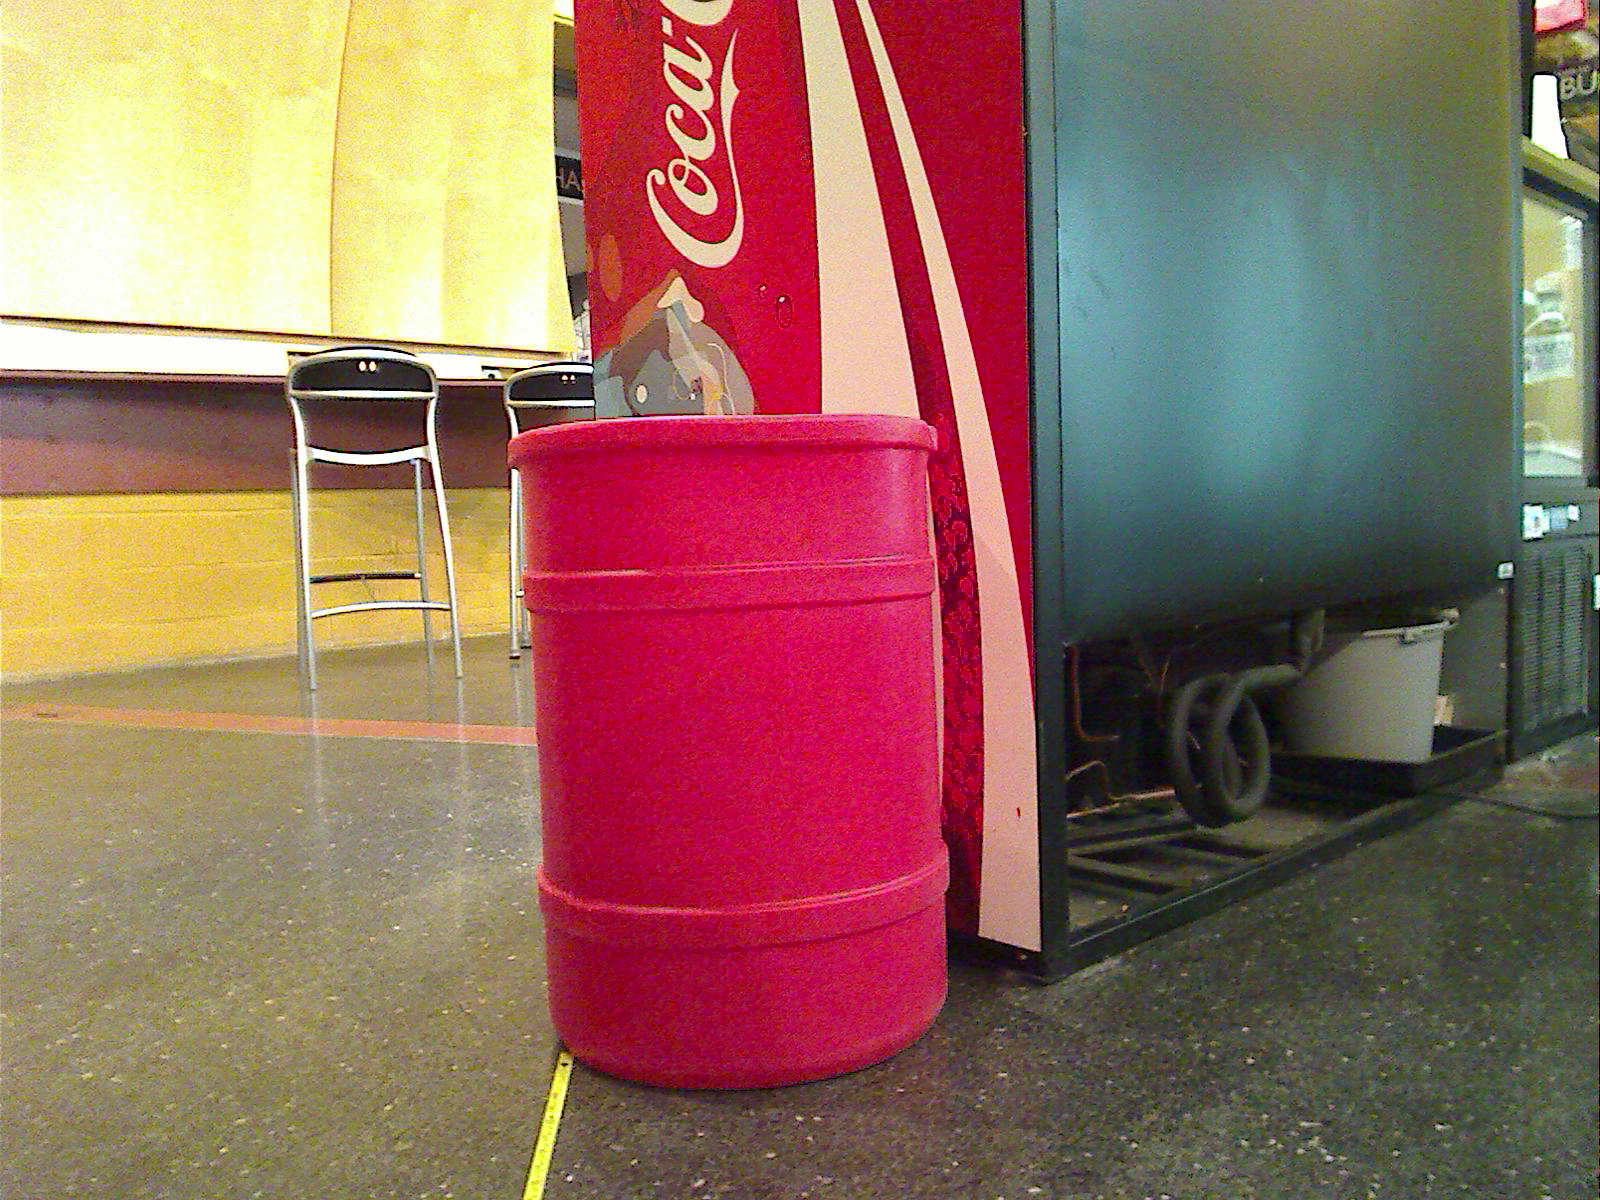
\includegraphics[width=0.4\columnwidth]{barrel_red.png}
%  \caption{Images under different lighting conditions. \label{fig:confusing}}
%\end{figure}

%----------------------------------------------------------------------------------------
%	METHODS
%----------------------------------------------------------------------------------------

\section{Methods}

%----------------------------------------------------------------------------------------
%	RESULTS
%----------------------------------------------------------------------------------------

\section{Discussion}

%----------------------------------------------------------------------------------------
%	REFERENCE LIST
%----------------------------------------------------------------------------------------

%\begin{thebibliography}{99} % Bibliography - this is intentionally simple in this template
%
%\bibitem[Figueredo and Wolf, 2009]{Figueredo:2009dg}
%Figueredo, A.~J. and Wolf, P. S.~A. (2009).
%\newblock Assortative pairing and life history strategy - a cross-cultural
%  study.
%\newblock {\em Human Nature}, 20:317--330.
%
%\end{thebibliography}

%----------------------------------------------------------------------------------------

\end{multicols}

\end{document}
